\section{Scope of the Thesis}

The focus of this thesis is centered on control systems utilized in safety-critical operations of Aerial robots. Our discussion pertains specifically to the challenges encountered by aerial robots operating in close proximity to static obstacles, such as buildings. We provide an in-depth analysis of the challenges faced by current state-of-the-art control systems and motivate towards the development of control algorithms in this context.


\subsection{Control Systems}

The application of control systems has been a pivotal aspect in the development of automation and robotics since the inception of the first robot in the 1950s. These systems are responsible for executing both low-level movements and high-level instructions in various systems, ranging from chemical plants to sophisticated dynamical robots. In the context of a robotic system, the controller assumes responsibility for governing the actions of the actuators while concurrently mitigating the discrepancy between the desired trajectory or position. This controller can be bifurcated into two distinct modules: firstly, the high-level controller, which formulates the requisite actuator torques or angles aimed at minimizing the position error, and secondly, the low-level controller, which diligently follows the desired torques or angles to accurately navigate the robot. The components of a robotic system are explained in Fig. \ref{robot_working_flowchart}. \\

\begin{figure}[h!]
    \centering
    \includegraphics[width=\columnwidth]{figures/intro/robot_working.png}
    \caption{Layout for an autonomous robotic system: The Controller works on a feedback loop to achieve desired system state given by the planner. }
    \label{robot_working_flowchart}
\end{figure}

These components are summarized below:

\begin{enumerate}
    \item The sensor stack supplies pertinent data regarding the environment to the processing unit, which in turn utilizes this information to develop a comprehensive comprehension of the surrounding which is leveraged by the planner.
    \item The Planner generates smooth trajectory points for the robot by avoiding obstacles to achieve the goal. These tasks can include reaching a goal location, or navigating from one place to another.  
    \item The High-level controller generates the desired actuator states using the desired trajectory as provided by the Planner. 
    \item The Low-level controller tracks the desired actuator states using a feedback loop which provides with the current actuator information after the robot dynamic system performs the given input.
\end{enumerate}

Although a planner defines a safe trajectory for a robot, a significant safety obstacle arises when the robot inaccurately tracks the trajectory or deviates from the intended path due to external disturbances. Consequently, ensuring stability and safety are primary concerns for any control system.

\subsection{Aerial Robots: Safety Critical Operations}

Unmanned Aerial Vehicles (UAVs) have been used for various tasks in the past decade. Present times have witnessed the widespread deployment of UAVs in numerous domains, ranging from delivery, search, and rescue to monitoring \cite{PEREZGRAU2021312, s20174708}. Some other tasks include surveillance, object detection, and civil infrastructure inspection. Civil inspection and delivery tasks necessitate close-range operations near stationary obstructions, such as bridges and buildings. Similarly, when a floating-base manipulator is attached to these UAVs, it can be utilized for various manipulation tasks \cite{Ciampa_2019, drones5040106, SREENATH2020656}. Aerial Manipulators (AMs) have gained much attention in recent years. The Unmanned Aerial Vehicle (UAV) acts as a floating base for the manipulator enabling it to conduct active operations in the 3D space. This combination of a UAV and a manipulator gives the system enough capabilities to perform complex operations where human access is limited (e.g., in disaster-affected zones) \cite{MOHDDAUD202230}. The other industrial and commercial applications of AMs are in the maintenance of power grids, the inspection of bridges, and canopy sampling.  \\

\begin{figure}[ht]
    \centering
    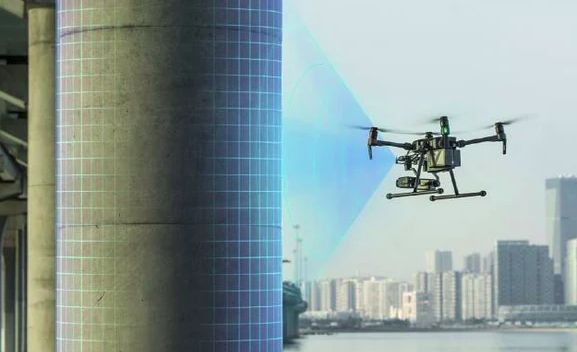
\includegraphics[width=0.6\textwidth]{figures/intro/Building_inspection.png}
    \caption[Shows current use of UAVs for inspection tasks near bridges.]{Shows current use of UAVs for inspection tasks near bridges. Source: \href{https://candrone.com/pages/inspection}{https://candrone.com/pages/inspection}}
    \label{}
\end{figure}

Such close proximity operations require maneuvering near these static obstacles \cite{drones6010005, drones7010045}. It is unarguable that any system designed for these applications must be contructed with safety in mind \cite{JEELANI2021105473}. 

In fact, safety has been a major hurdle in deploying such aerial manipulator systems in these applications \cite{WU2021103706}. The challenges faced in performing close proximity maneuvers are twofold: firstly, aerodynamic effects caused by ground, ceiling, and wall interference destabilize the drone and frequently result in collisions with obstacles \cite{gecesw, 8453469}; secondly, the highly coupled dynamics of the UAV and manipulator can generate undesirable forces and torques \cite{drones7020110, NALDI2018537}. Wind disturbances further exacerbate the situation by destabilizing the UAV and increasing the likelihood of collisions \cite{doi:10.1177/0020294019847688}.

\section{Research problems tackled}

\begin{enumerate}\label{enum:problems-addressed-by-thesis}
    \item[\textbf{A}] \textit{To design a control algorithm to incorporate safety guarantees for trajectory tracking of aerial robots.} \\
    
    A safety constraint needs to be imposed on the underlying controller to provide safety guarantees while flying in outdoor areas. These constraints should also tackle obstacle avoidance even when the desired trajectory is close to the obstacles. Hence, the controller needs to predict the external forces and the state of the robot in the next time steps to avoid obstacles safely. Hence, we develop a model predictive controller with constraints from Barrier lyapunov function which incorporates the predictive nature of the controller with obstacle avoidance constraints. 
    \\

    \item[\textbf{B}] \textit{To efficiently tackle non-linear dynamics of complex systems as an aerial manipulator in real-time.} \\
    
    Aerial manipulator is a combination of a floating manipulator attached on a UAV base. The coupled dynamics of such systems is non-linear which exerts many unwanted torques on the UAV making it unstable. To tackle this, the aerial manipulator model is given to the predictive controller which predicts these forces and gives control inputs. Similarly, modelling of robotic system enhances understanding of the system which in turn improves the stability.
    \\
    
    \item[\textbf{C}] \textit{To incorporate constraints to tackle external disturbances in the form of aerodynamic effects near static objects and strong winds in the high-level controller.} \\

    While operating near static obstacles, the aerial robot faces a lot of forces and torques due to the aerodynamic interactions of the rotor and the walls. These usually pull the robot towards the wall leading to collision and/or instability. Additional constraints to handle these forces must be incorporated to the underlying controller with disturbance rejection properties to handle these forces. This would also make the system disturbance tolerant for a bounded unmeasured disturbances. 
    \\
    
\end{enumerate}

\section{Motivation}

In this section, we discuss the various methods problems in earlier approaches of solving the research threads addressed in this thesis, which inspire certain aspects of our approach. We also mention alternative methods that might share similar inspiration or approaches but do not necessarily produce successful outcomes, and provide reasons for their shortcomings.

\subsection{Control of an Aerial Manipulator near static obstacles}

While the literature is sufficiently populated with novel design approaches of AMs, prior work involving safe control of the AM has been sparse \cite{8299552, 8350033, Meng2019SurveyOA}. Adaptive controllers \cite{7072729, 9213920} have been used to tackle torques due to the highly coupled dynamics of the AM by using an outer loop adaptive control over the proportional–derivative (PD) inner loop of the UAV. Though such strategies provide computational efficiency, they are incapable of incorporating constraints to avoid obstacles. Model Predictive Control (MPC) \cite{7991347,8594266, 9145644} significantly reduces the abruptness in control inputs and tracks the desired trajectory while anticipating future dynamic interactions of the AM. AMs also need to tackle impulsive torques whenever the arm tries to manipulate a object which further might lead to instability. 

Barrier Lyapunov functions (BLFs) \cite{8796030, 8581068} have been combined with MPC for obstacle avoidance of UAV as they can provide safety guarantees even in 3-dimensions. Safety is ensured by guaranteeing forward invariance of a safe region. BLF-based MPC \cite{9547384, 9655081} for a non-linear system have been proposed as stabilizing controllers to guarantee avoidance of a set of states associated with the unsafe region.

For operation near static obstacles, MPC \cite{9938397, 8887800, 8971725} has been utilized with hard constraints on the optimizer to avoid states which might lead to collision. These kinds of constraints don't incorporate velocity of the UAV and are not able to enforce the desired bound. Certain MPC algorithms have been formulated by incorporating these as soft constraints inside the MPC cost, which work satisfactorily when the constraint weight is high, but restrict the motion of the AM hindering effective trajectory tracking.

\begin{figure}[ht]
\centering
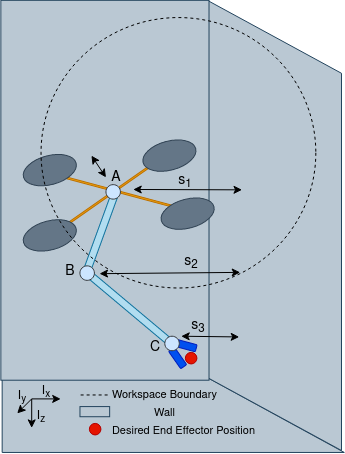
\includegraphics[width=0.4\columnwidth]{figures/AM/Drone_Problem_Formulation.png}
\caption{Image shows the Operation of an AM near 3 walls and the desired workspace for the AM.}
\label{paper_1_dig}
\end{figure}

We propose an MPC with constraints using BLF \cite{mundheda2022predictive, 8431468} , which provides safety guarantees while giving leeway to the MPC for effective trajectory tracking. It is also utilized to bind the AM into a safe region whenever obstacle positions are unknown. We modify the BLF earlier used for obstacle avoidance into a constraint for bounding the AM into a safe region. We also introduce a novel disturbance rejection term which prevents the AM from leaving the safe region and colliding with obstacles under external disturbances. The problem statement can be better understood as given in Fig. \ref{paper_1_dig}.


\subsection{Safe Maneuver of an Unmanned Aerial Vehicle inside a Tunnel}

Indoor operations of UAVs have been restricted due to the problems faced by UAVs near walls. Motion of a UAV in a tunnel has various challenges, primarily the aerodynamic effects due to the turbulent forces produced by the rotor and wall interactions. To account for such disturbances from all directions, we demonstrate our controller for operating inside a tunnel. 

Nonlinear Model Predictive Control (MPC) \cite{9145644} has been used for navigation and obstacle avoidance of UAVs for real-time utilities. MPC provides the predictive ability \cite{8594266} which aids in performing agile maneuvers with high precision and smooth control actions. \cite{9547384} tries to limit the risk of unsafety by formulating a probabilistic guarantee, but fails to provide a rigid safety guarantee to avoid obstacles. \cite{9938397} utilises partial sensor information to navigate through unknown environments by providing partial safety guarantees.  

Control Barrier Function (CBF) \cite{8796030} is used to guarantee safety-critical control for various domains, including dynamic robotic systems. \cite{8796030} introduces safety, safety sets, and describes using CBF to enforce safety in a minimally invasive fashion by not increasing the control effort or trajectory cost. CBF has been used as a constraint to MPC \cite{8887800} to provide safety guarantees while addressing the case of conflict between safety and performance. This provides improved performance to MPC while providing safety guarantees. \cite{9655081} shows collision avoidance for multi UAV swarm to reach desired locations and providing safety guarantees. \cite{mundheda2022predictive} utilizes MPC while handling external wind disturbances. 
Although nonlinear controllers have been tried separately for ground and ceiling effects, no effort has been made to minimize the impacts of these disruptions using a disturbance resistive barrier function. 

\begin{figure}[ht]
    \centering
    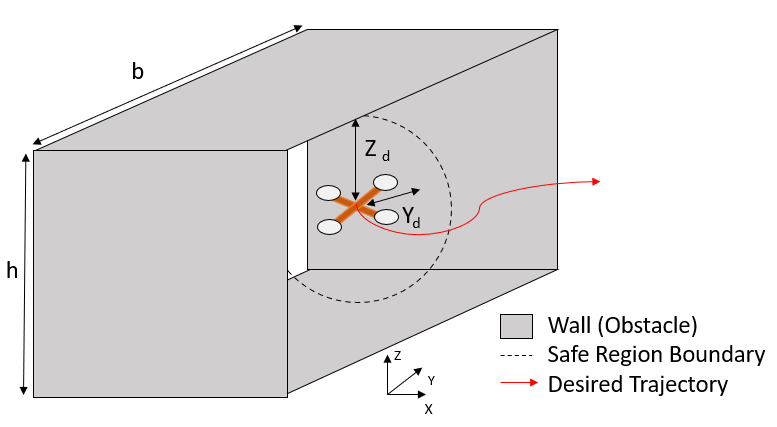
\includegraphics[width=0.7\textwidth]{figures/UAV/problem.png}
    \caption{Image shows the trajectory tracking of a UAV inside a tunnel while handling aerodynamic effects from the walls.}
    \label{problem_def_2_intro}
\end{figure}

We tackle disturbances due to aerodynamic interactions with wall by modifying the BLF. This modified constraint is added to the MPC controller which provides smooth trajectories even in the presence of unknown bounded disturbances. The problem statement can be better understood as given in Fig. \ref{problem_def_2_intro}.

\section{Contributions}

This thesis provides the following contributions:

\begin{enumerate}
    \item To the best of the author's knowledge, this is the first attempt to design a predictive controller with constraints for Barrier Lyapunov Function (BLF) for an aerial manipulator.
    \item The proposed controllers provide obstacle avoidance to the aerial robots while achieving tangible performance gain over existing predictive controllers.
    \item We exploit the BLF to create a novel constraint to bound the UAV inside inside a defined safe boundary, which is contrary to it's earlier avoidance utility.
    \item For a UAV, the proposed controller is the first attempt to handle all three effects (ground, ceiling, and wall).
    \item We also introduce changes to the BLF to tackle external bounded wind disturbances by a distance rejection term.
\end{enumerate}

\section{Thesis Layout}

\begin{itemize}
    \item[C1] This chapter discusses the scope of this thesis describing the research problem tackled in terms of control systems for aerial robots. We outline the motivation behind the research problem and techniques others use for similar problems. 
    \item[C2] In this chapter, we present the background on the dynamics of aerial robots, state space models, Model Predictive Control, and Barrier Lyapunov function. We explain how to formulate these for our proposed controller and provide details on their use.  
    \item[C3] This chapter is the first contribution of this thesis. We demonstrate MPC-BLF as predictive control algorithms for an aerial manipulator with the ability to avoid obstacles and enclose the aerial manipulator in a confined safe space. 
    \item[C4] In this chapter, we contribute to algorithm development for maneuvering a UAV through a tunnel and handling additional aerodynamic torques from interactions with the tunnel walls.
    \item[C5] In this chapter, we present the conclusion for the thesis with future prospects and endeavors. The thesis also proposes directions for newer research and practical use cases of the proposed algorithms. 
\end{itemize}

